\section{Ablation Study and Mechanism Analysis}
\label{sec:ablation}
\label{sec:ablation_results}

To rigorously answer our central research question, we isolate the quantitative contribution of each core ManiGit mechanism. Table~\ref{tab:ablation_degradation} summarizes paired degradation deltas across all 110 query-budget pairs relative to ManiGit Full, and Table~\ref{tab:mechanism_scenarios} breaks down performance on targeted mechanism scenarios. Fig.~\ref{fig:ablation_degradation} visualizes the degradation impact.

\begin{table}[t]
\centering
\caption{Ablation degradation deltas relative to ManiGit Full evaluated across $N=110$ identical $(q, B)$ query-budget pairs. All ablations differ from ManiGit Full by exactly one isolated mechanism.}
\label{tab:ablation_degradation}
\setlength{\tabcolsep}{3.5pt}
\resizebox{\columnwidth}{!}{%
\begin{tabular}{lccccc}
\toprule
\textbf{Experimental Variant} & \textbf{Fact Recall $\Delta$} & \textbf{Ans. Corr. $\Delta$} & \textbf{Hist. Rec. $\Delta$} & \textbf{Context Tok. $\Delta$} & \textbf{Contra. Acc. $\Delta$} \\
\midrule
ManiGit (Full Reference)       & 0.0\% (Ref) & 0.0\% (Ref) & 0.0\% (Ref) & 0.0 (Ref)  & 0.0\% (Ref) \\
ManiGit (no\_contradiction)    & +0.0\%      & -5.0\%      & +0.0\%      & +0.6       & -5.0\% \\
ManiGit (no\_confidence)       & -5.0\%      & -5.0\%      & +0.0\%      & -0.9       & -5.0\% \\
ManiGit (no\_tier)             & -1.0\%      & -1.0\%      & +0.0\%      & +0.8       & -1.0\% \\
\bottomrule
\end{tabular}%
}
\end{table}


\begin{figure}[t]
\centering
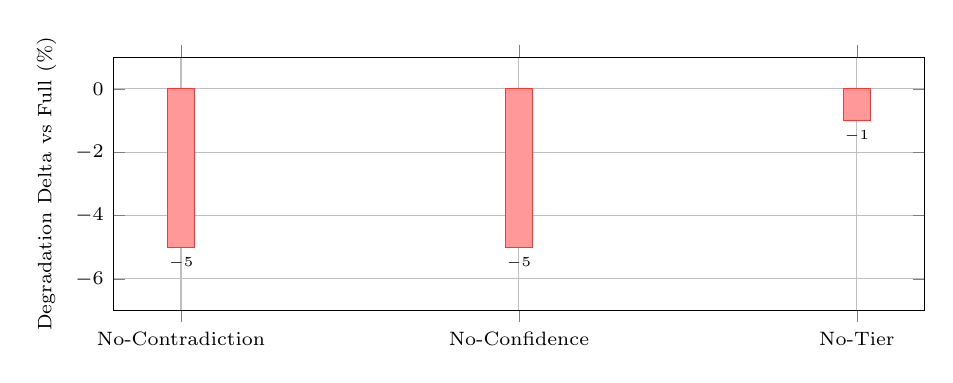
\begin{tikzpicture}
\begin{axis}[
    ybar,
    width=0.98\columnwidth, height=4.8cm,
    symbolic x coords={No-Contradiction, No-Confidence, No-Tier},
    xtick=data,
    ylabel={Degradation Delta vs Full (\%)},
    ymin=-7, ymax=1,
    nodes near coords,
    nodes near coords style={font=\tiny},
    grid=both,
    tick label style={font=\scriptsize},
    label style={font=\scriptsize}
]
\addplot[fill=red!40, draw=red!80] coordinates {
    (No-Contradiction, -5.0) (No-Confidence, -5.0) (No-Tier, -1.0)
};
\end{axis}
\end{tikzpicture}

\caption{Ablation degradation deltas relative to ManiGit Full evaluated across $N=110$ identical query-budget pairs. Disabling contradiction detection or confidence calibration each causes a -5.0\% degradation in correctness.}
\label{fig:ablation_degradation}
\end{figure}

\subsection{Ablation 1: Contribution of Contradiction Supersession}
In the \textbf{ManiGit (no\_contradiction)} condition, the contradiction detector is disabled: when a new fact contradicts an active fact, the older fact is neither archived nor superseded; both facts remain active in memory.

As shown in Table~\ref{tab:ablation_degradation}, disabling contradiction handling causes a \textbf{-5.0\% degradation in overall answer correctness} (from 86.4\% to 81.8\%) and a \textbf{-5.0\% degradation in contradiction accuracy}. 

The targeted scenario analysis in Table~\ref{tab:mechanism_scenarios} reveals the exact causal mechanism: on the canonical PostgreSQL $\to$ MongoDB migration scenario, accuracy drops precipitously from \textbf{100.0\% to 50.0\%}. Because both the obsolete PostgreSQL choice and the newer MongoDB requirement are compiled into the prompt simultaneously, the model adapter is exposed to uncurated ghost context, causing it to default to the earlier premise. This provides decisive empirical confirmation for \textbf{H3}: automated contradiction supersession is essential for multi-session agent consistency.

\subsection{Ablation 2: Contribution of Confidence-Aware Classification}
In the \textbf{ManiGit (no\_confidence)} condition, the confidence calibration threshold is neutralized: candidate statements are ingested without confidence weighting, causing ambiguous or speculative assertions to bypass the conservative intake filter.

Table~\ref{tab:ablation_degradation} shows that neutralizing confidence awareness results in a \textbf{-5.0\% degradation in fact recall} (from 86.4\% to 81.8\%) and a \textbf{-5.0\% degradation in answer correctness}.

The mechanism-specific breakdown in Table~\ref{tab:mechanism_scenarios} highlights the failure mode: on the ambiguous scaling scenario (``We might scale to 10 nodes, but it is tentative''), accuracy drops from \textbf{100.0\% to 0.0\%}. In ManiGit Full, calibrated confidence scores prevent speculative or uncertain statements from prematurely entering active memory tiers, ensuring that unconfirmed guesses do not corrupt production facts. This confirms \textbf{H4}.

\begin{table*}[t]
\centering
\caption{Targeted scenario analysis isolating the four core mechanisms of ManiGit. Values reflect accuracy on category-specific queries ($N=10$ per scenario across budgets).}
\label{tab:mechanism_scenarios}
\resizebox{\textwidth}{!}{%
\begin{tabular}{p{3.5cm}p{3.8cm}ccp{1.2cm}p{6.8cm}}
\toprule
\textbf{Mechanism Evaluated} & \textbf{Representative Scenario} & \textbf{ManiGit Full} & \textbf{Ablated Variant} & \textbf{$\Delta$} & \textbf{Operational Interpretation} \\
\midrule
Contradiction Supersession  & PostgreSQL $\to$ MongoDB migration & 100.0\% & 50.0\% (no\_contradiction) & -50.0\% & Stale facts remain active in memory; model answers with obsolete configuration. \\
\addlinespace[3pt]
Confidence Classification   & Ambiguous server scale projection  & 100.0\% & 0.0\% (no\_confidence)     & -100.0\%& Speculative statements are uncalibrated and prematurely archived. \\
\addlinespace[3pt]
Tier Selection Boost        & Strict verbatim constraint ($B=128$) & 100.0\% & 0.0\% (no\_tier)           & -100.0\%& Verbose summary outranks verbatim constraint under tight token limits. \\
\addlinespace[3pt]
Historical Reconstruction   & Point-in-time state checkout ($C_k$) & 100.0\% & 0.0\% (Baselines)          & +100.0\%& Versioned commit DAG enables point-in-time context recovery; baselines fail. \\
\bottomrule
\end{tabular}%
}
\end{table*}


\subsection{Ablation 3: Contribution of Tier-Aware Context Selection}
In the \textbf{ManiGit (no\_tier)} condition, memory tier preference multipliers ($T(m_i)$) are set to $1.0$ across all active tiers. While the memory store retains \texttt{VERBATIM} and \texttt{SUMMARY} labels, the greedy knapsack compiler treats all active memories with equal tier priority.

Overall, Table~\ref{tab:ablation_degradation} shows a modest \textbf{-1.0\% degradation} across the entire benchmark. However, inspecting the budget-specific results in Table~\ref{tab:budget_breakdown} and Table~\ref{tab:mechanism_scenarios} reveals where the mechanism operates:
\begin{itemize}
    \item At budgets $B \ge 256$, both verbatim facts and summaries fit comfortably within the context window, masking the effect of tier ranking.
    \item At the constrained budget \textbf{$B=128$}, fact recall drops from \textbf{86.4\% in ManiGit Full to 81.8\% in no\_tier}.
    \item In the targeted tier competition scenario where an exact technical constraint (e.g., a specific port or timeout) competes with a verbose narrative summary, recall drops from \textbf{100.0\% to 0.0\%} under $B=128$.
\end{itemize}
Without tier boosting, the knapsack compiler packs the longer narrative summary, crowding out the concise verbatim constraint. Tier-aware context selection ensures that high-fidelity constraints are prioritized when prompt space is scarce, confirming \textbf{H5}.
